\subsection{Disk Arrangements}
It turns out the disk arrangements are an equivalent way to to represent plane graphs.  By 
representing vertices as interioir disjoint disks and by representing edges as as points of 
intersections (contact), \textit{kissing 
points} between two disks.  The graph corresponding to a given disk arrangement, $\DD$, is said to 
be the \textit{contact graph}. A \it{disk arrangement} is a set, $\DD$, of pairwise 
interior-disjoint disks in the plane, 
$\DD=\left\lbrace C_i \right\rbrace_{i = 1}^n $.
$\left\lbrace C_i \right\rbrace_{i = 1}^n $ such that for any circle $C \in \left\lbrace C_i 
\right\rbrace_{i = 1}^n$, $C$


%(fig 1) a disk arrangement
%(fig 2) an equivalent contact graph to (fig 1)
A classical result by Thurston and Koebe is that every disk arrangement embedded into the plane had 
a corresponding plane graph.
\begin{thm}[\ref{stephenson2005introduction}Disk Packing Theorem]\label{thm2-1}
For every graph $G$, there is a disk arrangement in the
plane whose contact graph is isomorphic to $G$.
\end{thm}

%add a paragraph with atoms of molecules are modeled with disks and balls of fixed radii. The 
%if two disks are in contact, then the  distance between their centers  = the sum of the radii
%conclude: disk arrangements are better models for representing atoms and molecules fixed distance 
% betweeen atoms
\begin{prop}
 For every linkage $L$, there is a disk arrangement in the
plane whose contact graph is isomorphic to $L$.
\end{prop}


\begin{figure}[h]
\begin{center}
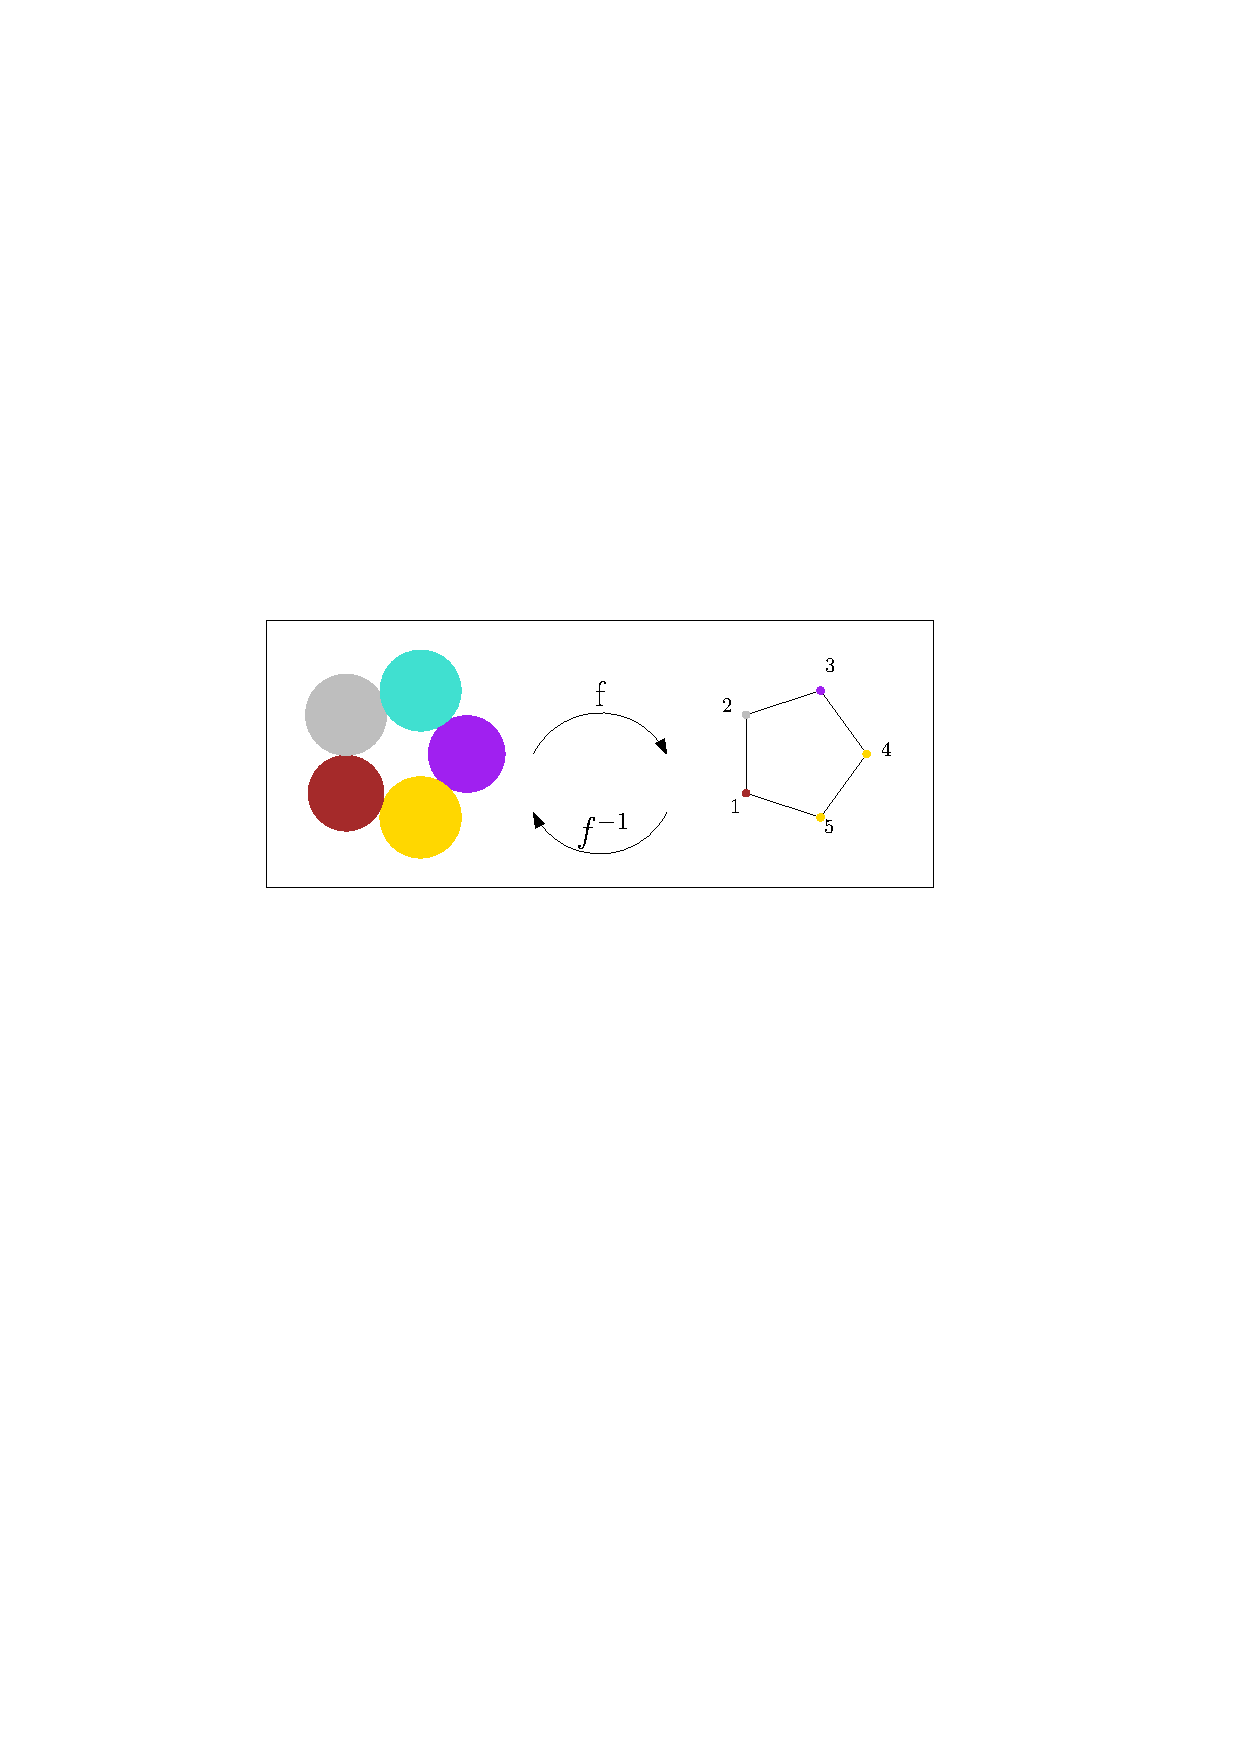
\includegraphics[scale=1]{graphics/diskPackingTheoremExample.pdf}
\end{center} 
\caption{This example represents a disk arrangement transformed to and from its corresponding graph 
$G_2$}
\label{fig:DiskArrangement-1}
\end{figure}
\begin{enumerate}%1,2,3,4....
%\item Introduce the circle packing theorem.
\item Show the relation between polygonal linkages and disk arrangengements.
\end{enumerate} 
\subsubsection{Ordered Disk Arrangement}
Suppose we're given a tree. By the disk packing theorem we can ascertain a sense of order for the 
isomorphic disk packing.  An \textit{ordered disk arrangement} is a rooted tree in which the 
counter-clockwise ordering of adjacent vertices.
\subsubsection{Disk Packing Confinement Problem}
Given inputs of radii 
By adding constraints to the embeddings of disk arrangements, we can devise realizability problem 
by a volume argument.
\begin{enumerate}%1,2,3,4....
\item Round 1: Start with a disk of unit radius.
\item Round 2: Add two kissing disks, each of diameter 2, that do not intersect with any other 
disk (they 
may kiss other
disk).
\item Round 3 and Higher: For each new kissing disk added, add two more non-intersecting kissing 
disks of diameter 2 to it.
\end{enumerate} 
For each round $i$ we are adding $2^{(i-1)}$ disks, each with an of $\pi$.  The area that 
the disk arrangement is bounded by at round $i$ is a box of length $2\cdot (2\cdot (i-1)+1)$ 
totalling to an area of $(4\cdot i^2 - 4\cdot i + 1)$.  Meanwhile the total area of the disk 
arrangement at round $i$ is $\pi \cdot (2^i - 1)$.  The exponential growth rate of the disk packing 
will exceed its bounded area for sufficiently large $i$.

Figure (\ref{fig:circlePacking-1}) illustrates the iterative problem.  The problem with this is that 
the area in
which is necessary to contain this disk growing disk arrangement will exceed the area needed to 
contain it.
\begin{figure}[H]
\begin{center}
    %add desired spacing between images, e. g. ~, \quad, \qquad etc.
    %(or a blank line to force the subfigure onto a new line)
  \begin{subfigure}[b]{0.24\textwidth}
	  
\includegraphics[width=\textwidth]{graphics/degree2arrangement.pdf}
	  \caption{A disk arrangement with two layers of disks}
	  \label{fig:circlePacking1-1}
  \end{subfigure}
  \begin{subfigure}[b]{0.24\textwidth}
	  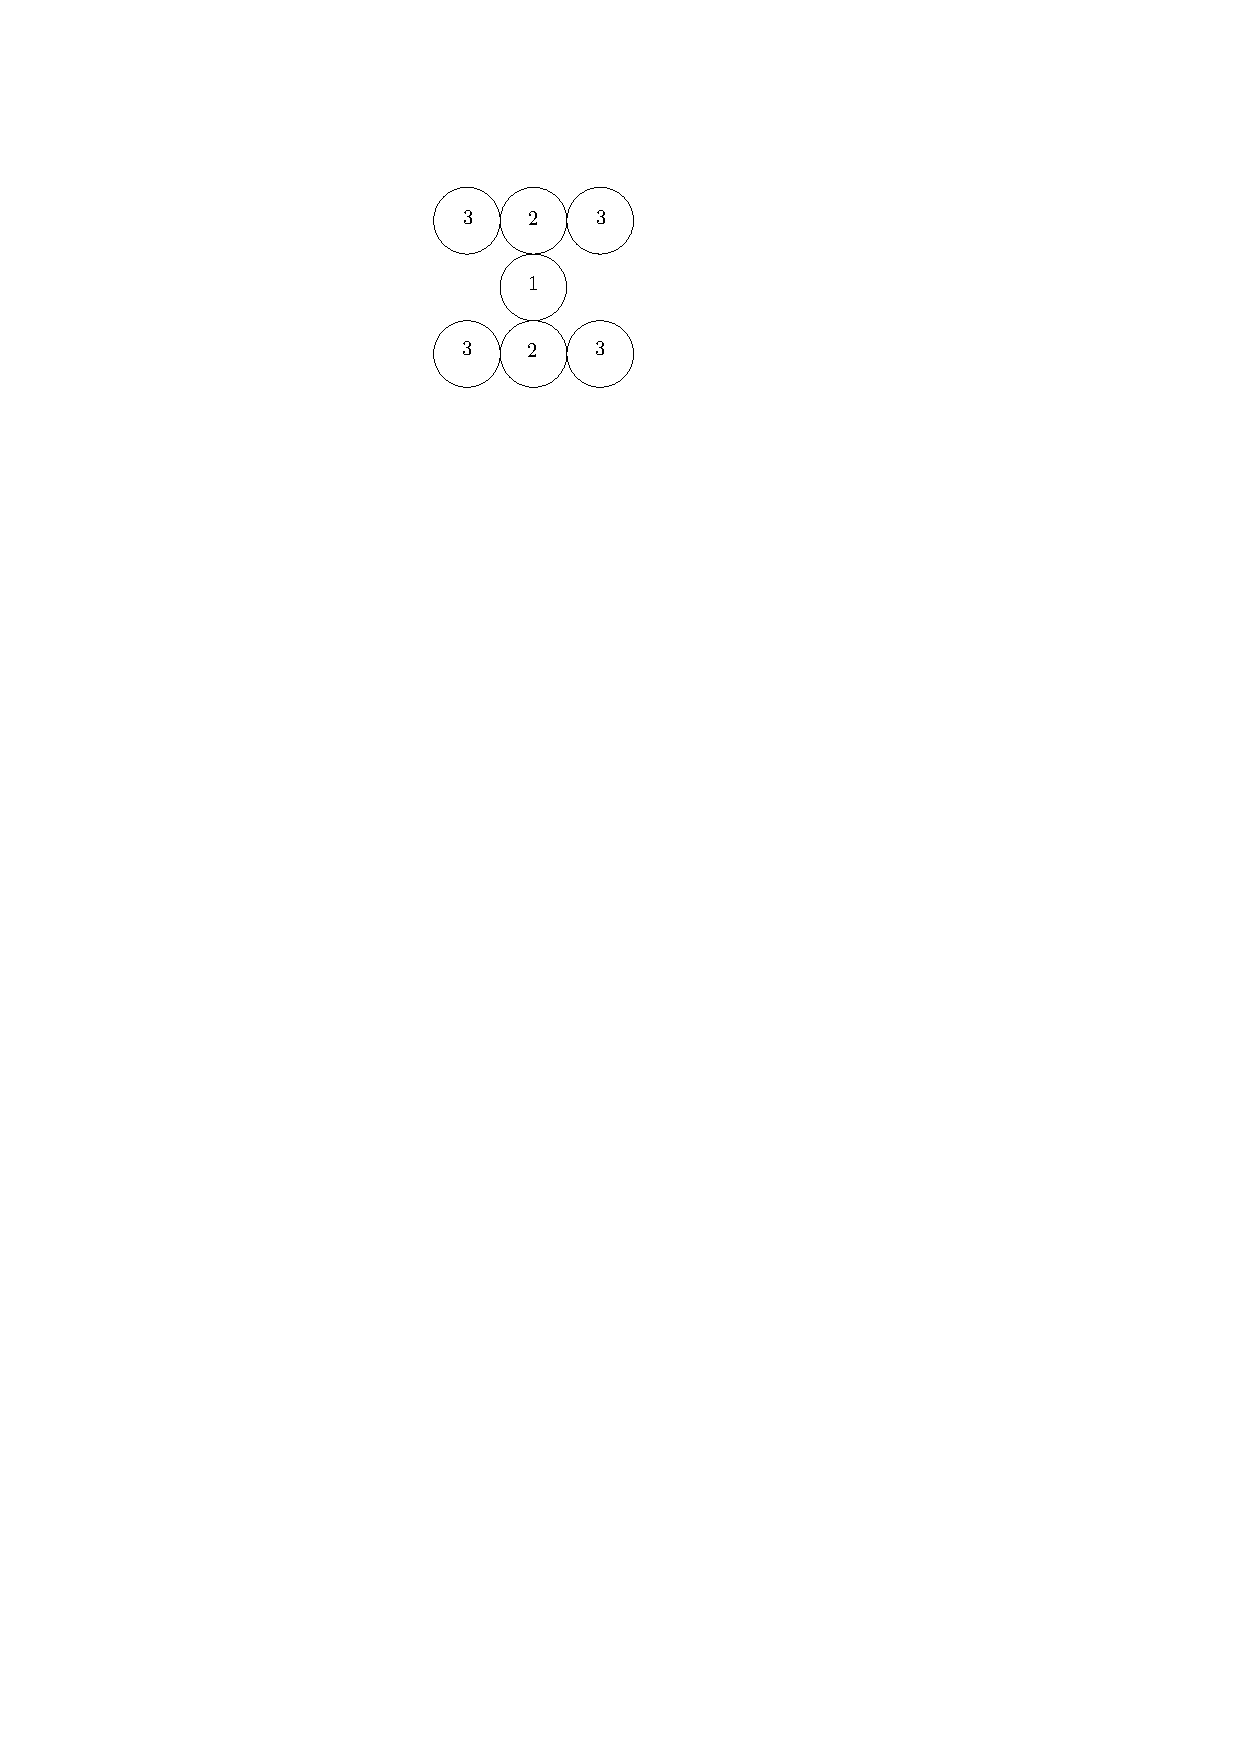
\includegraphics[width=\textwidth]{graphics/degree3arrangement.pdf}
	  \caption{A disk arrangement with three layers of disks}
	  \label{fig:circlePacking1-2}
  \end{subfigure}
  \begin{subfigure}[b]{0.24\textwidth}
	  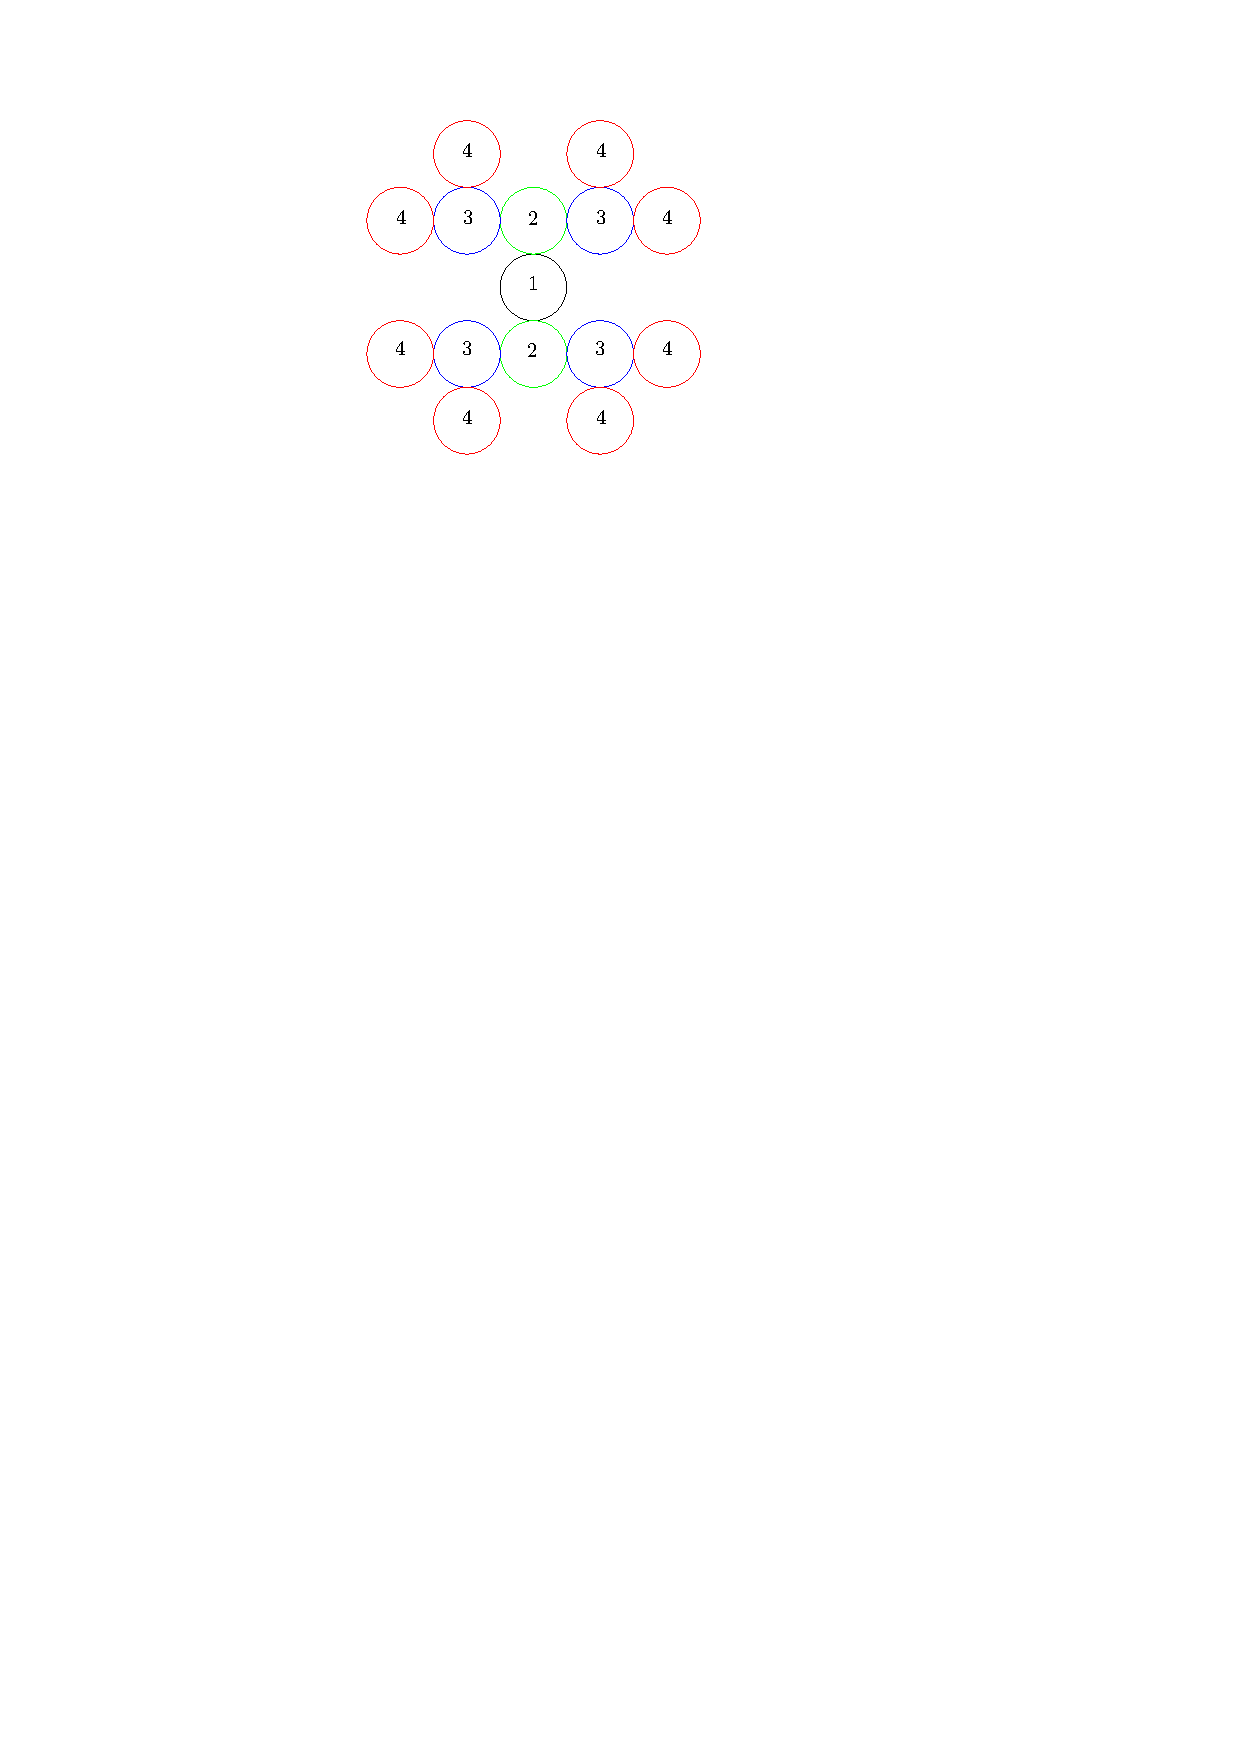
\includegraphics[width=\textwidth]{graphics/degree4arrangement.pdf}
	  \caption{A disk arrangement with four layers of disks}
	  \label{fig:circlePacking1-3}
  \end{subfigure}
  \begin{subfigure}[b]{0.24\textwidth}
	  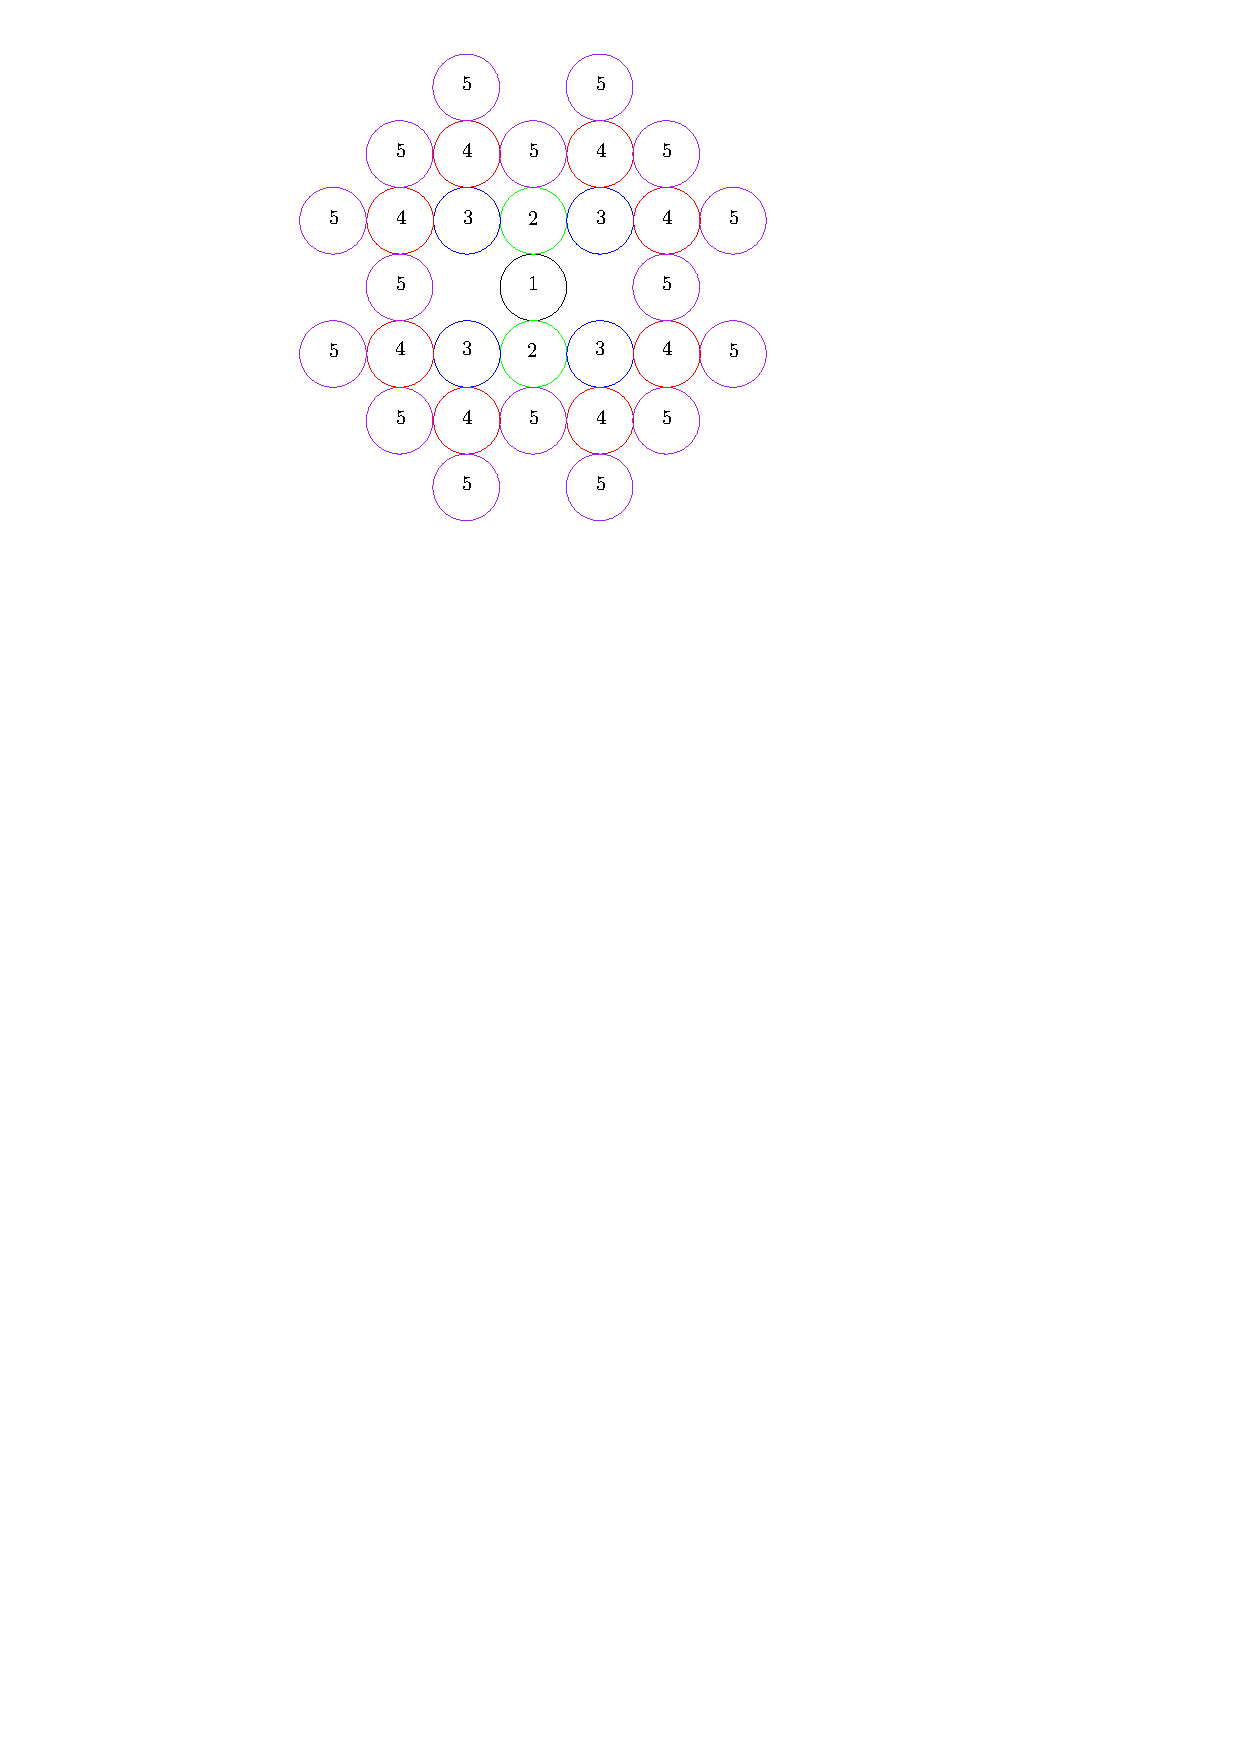
\includegraphics[width=\textwidth]{graphics/degree5arrangement.pdf}
	  \caption{A disk arrangement with five layers of disks}
	  \label{fig:circlePacking1-3}
  \end{subfigure}
\end{center} 
\caption{The gradual growth of disk arrangements by adding two kissing disks to each of the 
previously generated disks.  By continuing this arrangement growth, the space needed to contain the 
kissing disks will exceed the area containing the disk arrangements.}\label{fig:circlePacking-1}
\end{figure}
